\section{Week 2}
\textbf{\large Time Constants}
\begin{align*}
    \frac{1}{\tau s + 1} &\xrightarrow{\mathcal{L}^{-1}} e^{-\frac{1}{\tau} t} \to \; \text{smaller $\tau$, faster response} \\
    \frac{1}{s + a} &\xrightarrow{\mathcal{L}^{-1}} e^{-a t} \to \; \text{greater $a$, faster response}
\end{align*}

\textbf{\large Settling Time}
\begin{align*}
    t_s &= \frac{\ln(1-0.95)}{-a} \approx \frac{3}{\sigma} \\
    t_s &= \frac{\ln(1-0.98)}{-a} \approx \frac{4}{\sigma}
\end{align*}

\textbf{\large Second-order system damping ratio}
\begin{figure}[H]
    \centering
    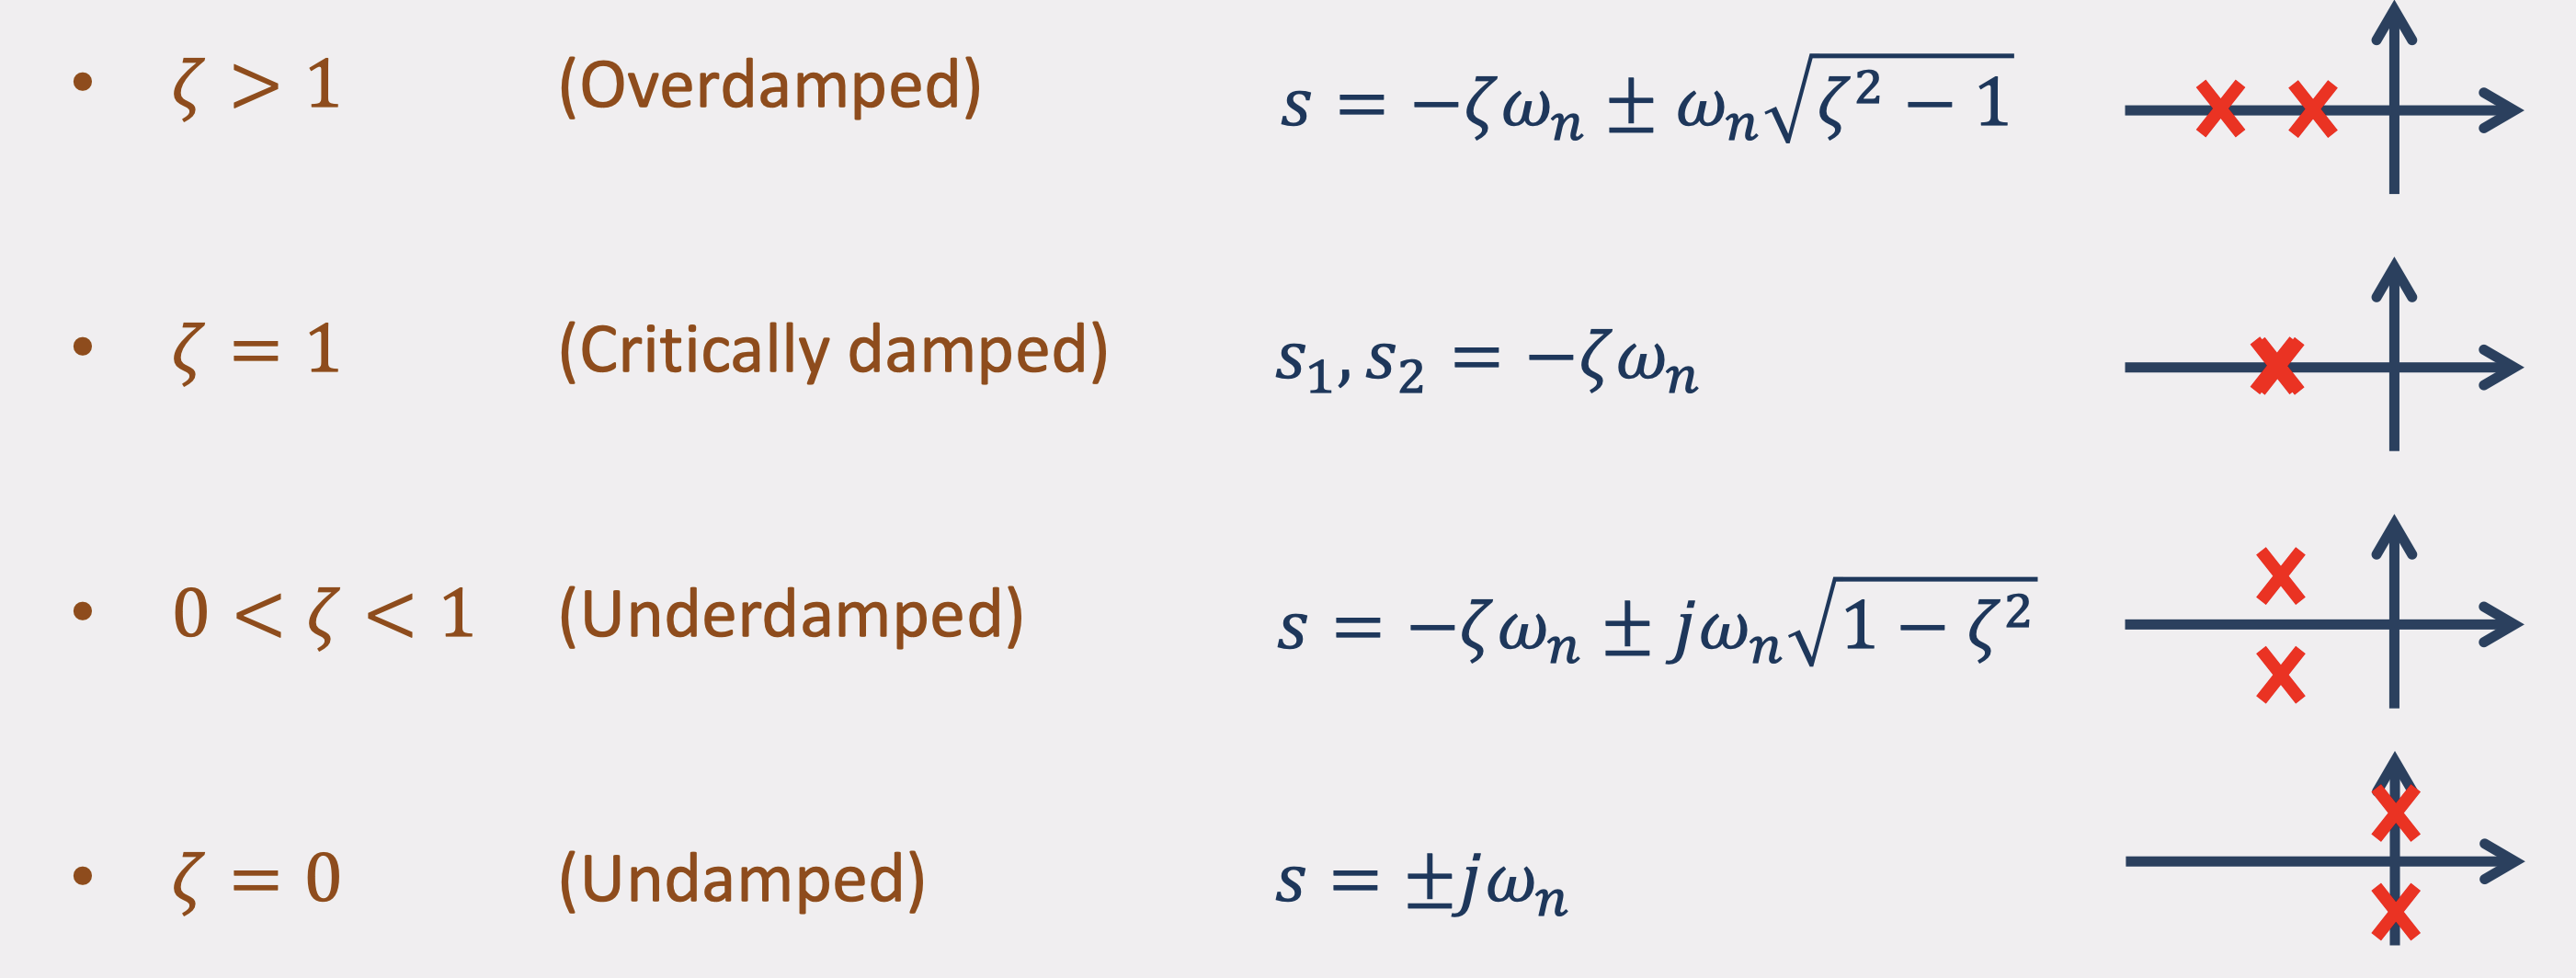
\includegraphics[width=0.45\textwidth]{images/damping_ratio.png}
\end{figure}
\vspace{1cm}

\textbf{\large S-plane parameters}
\begin{figure}[H]
    \centering
    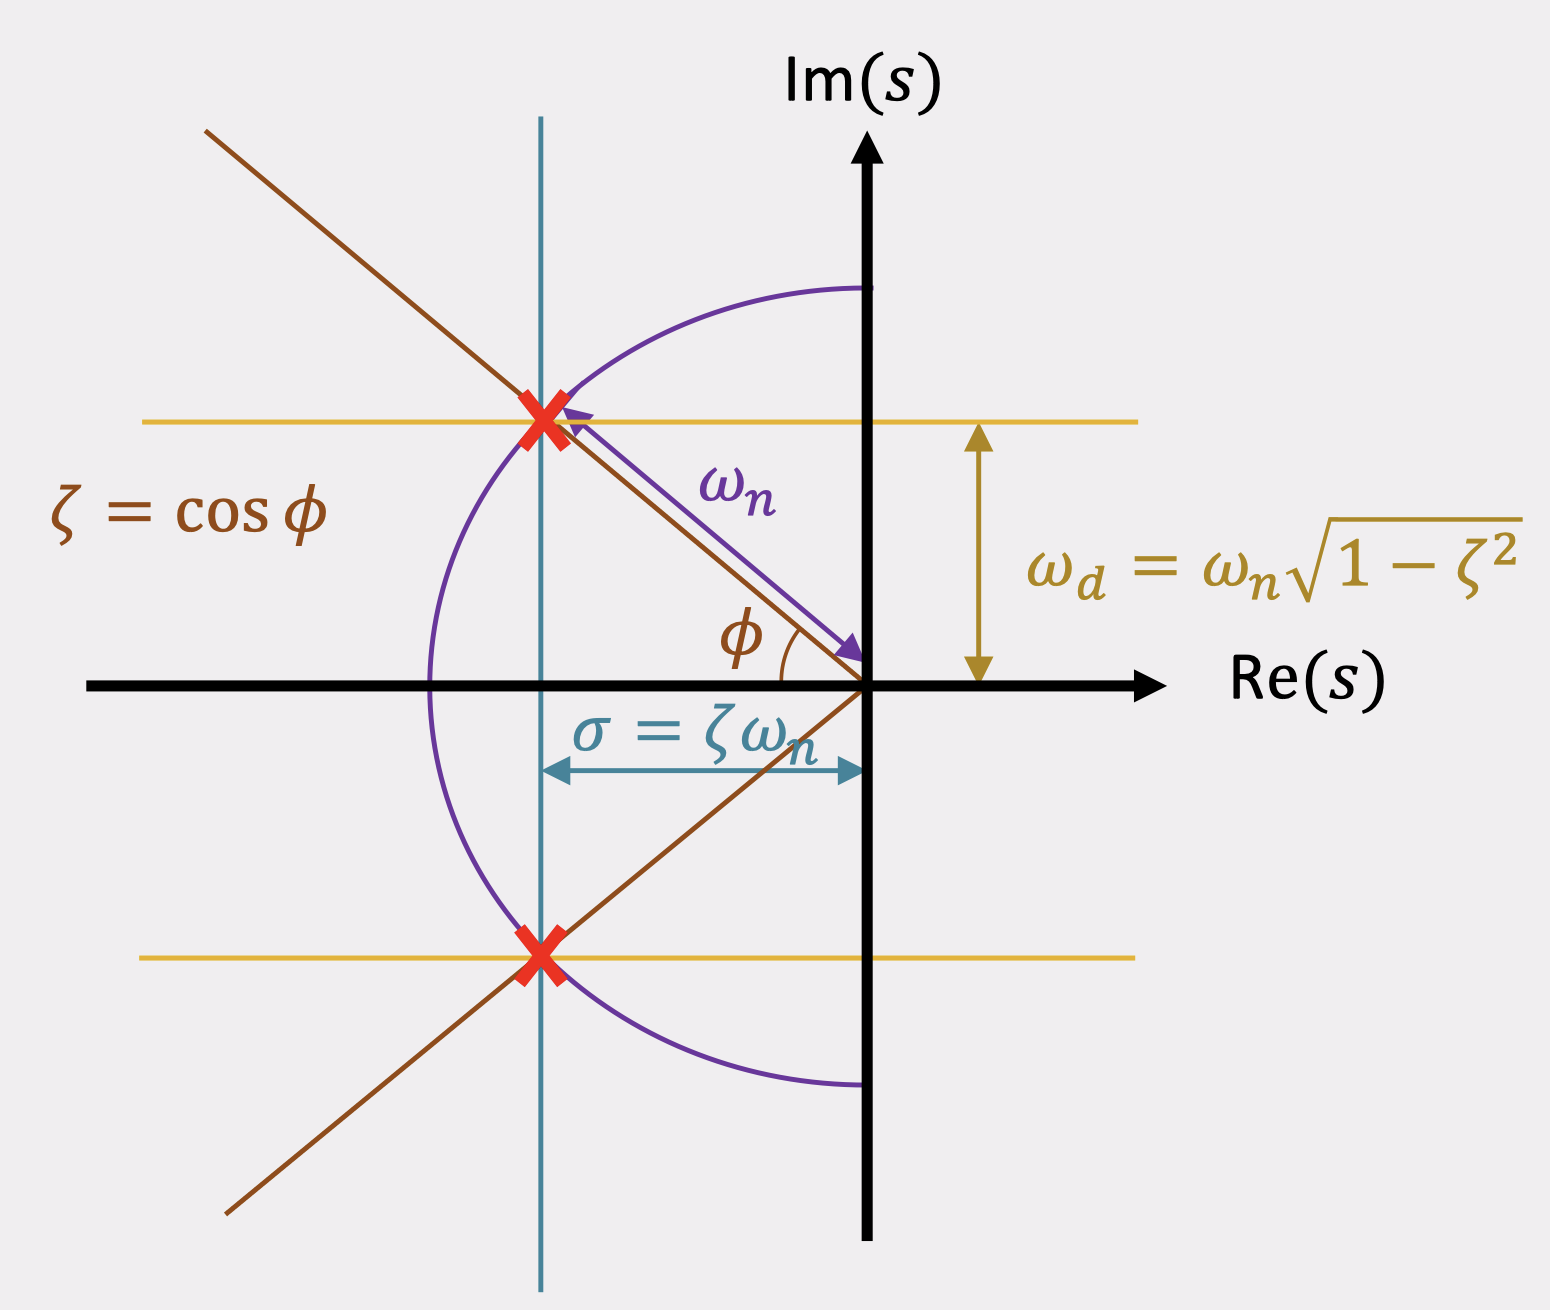
\includegraphics[width=0.45\textwidth]{images/s_plane_parameters.png}
\end{figure}

\textbf{\large Steady state gains}
\begin{itemize}
    \item \textbf{\underline{DC gain:}} 
    
    steady state of the unit step response.
    \begin{equation*}
        \text{DC Gain} = \lim_{s\to 0} G(s) 
    \end{equation*}
    \item \textbf{\underline{Instantaneous Gain:}} 
    
    initial value of the unit step response. 
    
    \textbf{All physical system should have zero Inst. Gain}.
    \begin{equation*}
        \text{Inst. Gain} = \lim_{s\to\infty} G(s)
    \end{equation*}
\end{itemize}


 

\textbf{\large Properness}
\begin{equation*}
    G(s) = \frac{s^n + a_{n-1}s^{n-1}+a_{n-2}s^{n-2}+\ldots + a_0}{s^m + b_{m-1}s^{m-1}+b_{m-2}s^{m-2}+\ldots + b_0}
\end{equation*}
\begin{itemize}
    \item \textbf{strictly proper when $m > n$ .} \\ Most physical/real system are strictly proper.
    \item \textbf{proper when $m = n$ .} \\ Discrete system (computer) is proper.
    \item \textbf{improper when $m < n$ .} \\ Cannot be physically implemented. Because in order to deliver a control signal \textbf{now}, you need to know a \textbf{future} input value.
\end{itemize}

